\chapter{Practical part}
The practical part of my thesis was to create a plug-in for the visualization application ``Volumeshop `` that was developed at the Computer graphics institute at TU Wien. I built my work upon an Existing plug-in, that split meshes in image space.
\section{Plan and milestone definition:}
The practical part was split into three milestones containing the following tasks:
\begin{itemize}
\item \textbf{Milestone 1} \emph{Selection of split meshes, selected parts are not split and stay in place} Make a simple, intuitive but manual way of creating exploded Views.
\item \textbf{Milestone 2} \emph{Find a safe distance, find a split plane} Automatize the creation of the visualization, by automatically finding a split plane and an offset.
\item \textbf{Milestone 3} \emph{Optimize Distance, force-field animation of split, optimize fringe distance cases} Make the visualization more pleasant to look at by adding a seemingly antural force-field animation and prevent unnecessary large offsets by introducing ghosting techniques.
\end{itemize}
\section {Tools and languages}
Since the project is based upon an existing framework, I used its languages, c++ for the main program and the GLSL for the openGL shaders.
\section{Documentation of the implementation each milestone}
\subsection{Milestone 1:Selection of split meshes, selected parts are not split and stay in place} The original plug-in drew split meshes by drawing them twice, with a manually defined offset, from a manually defined split plane. The fragment shader then rejects fragments that were behind or in front of the also translated split plane, rendering them in a predetermined fashion.\\
The first step towards an exploded view was now to use the already implemented group selection feature to define an object of interest that would not be split or translated like the rest of the mesh. To realize this I introduced a third rendering of the mesh in the display function. This render pass would render only the object of interest in its original location in the non-displaced mesh.\\
This also required that the ``renderMesh''-function be modified, introducing a new boolean parameter ``split'' that tspecifies, if the object is rendered in split mode, or in the ``object-of-interest-mode''. When the function loops through the groups of a mesh, it checks if the the group is in the group . If that is the case and the function parameter ``split'' is false, the group will be rendered. If split is false and the group is not selected, it will also be drawn, this time displaced.\\
Also a new option ``split'' for the shader was introduced, given that there is no need to pass an offset or split plane to render the object of interest. This basically reverts the fragment shader to the original trianglemesh-shader\\
After that was done an exploded view of the object was now rendered with manual definition of the offset and split plane with one usability glitch: A colour picking algorithm was already implemented, but it didn't consider the splitting and translation of the object. This resulted in a behaviour where clicking on a part of the object when it was split would cause false selection or deselection. \\
To set this right, I modified the the overlay function so that it would also be rendered three times like the normal rendering, modifying the ``renderGroup'' function once more  so that it could also render the overlay function and adding an ``overlay''option to the shader.
\begin{figure}[tb]
	\centering
	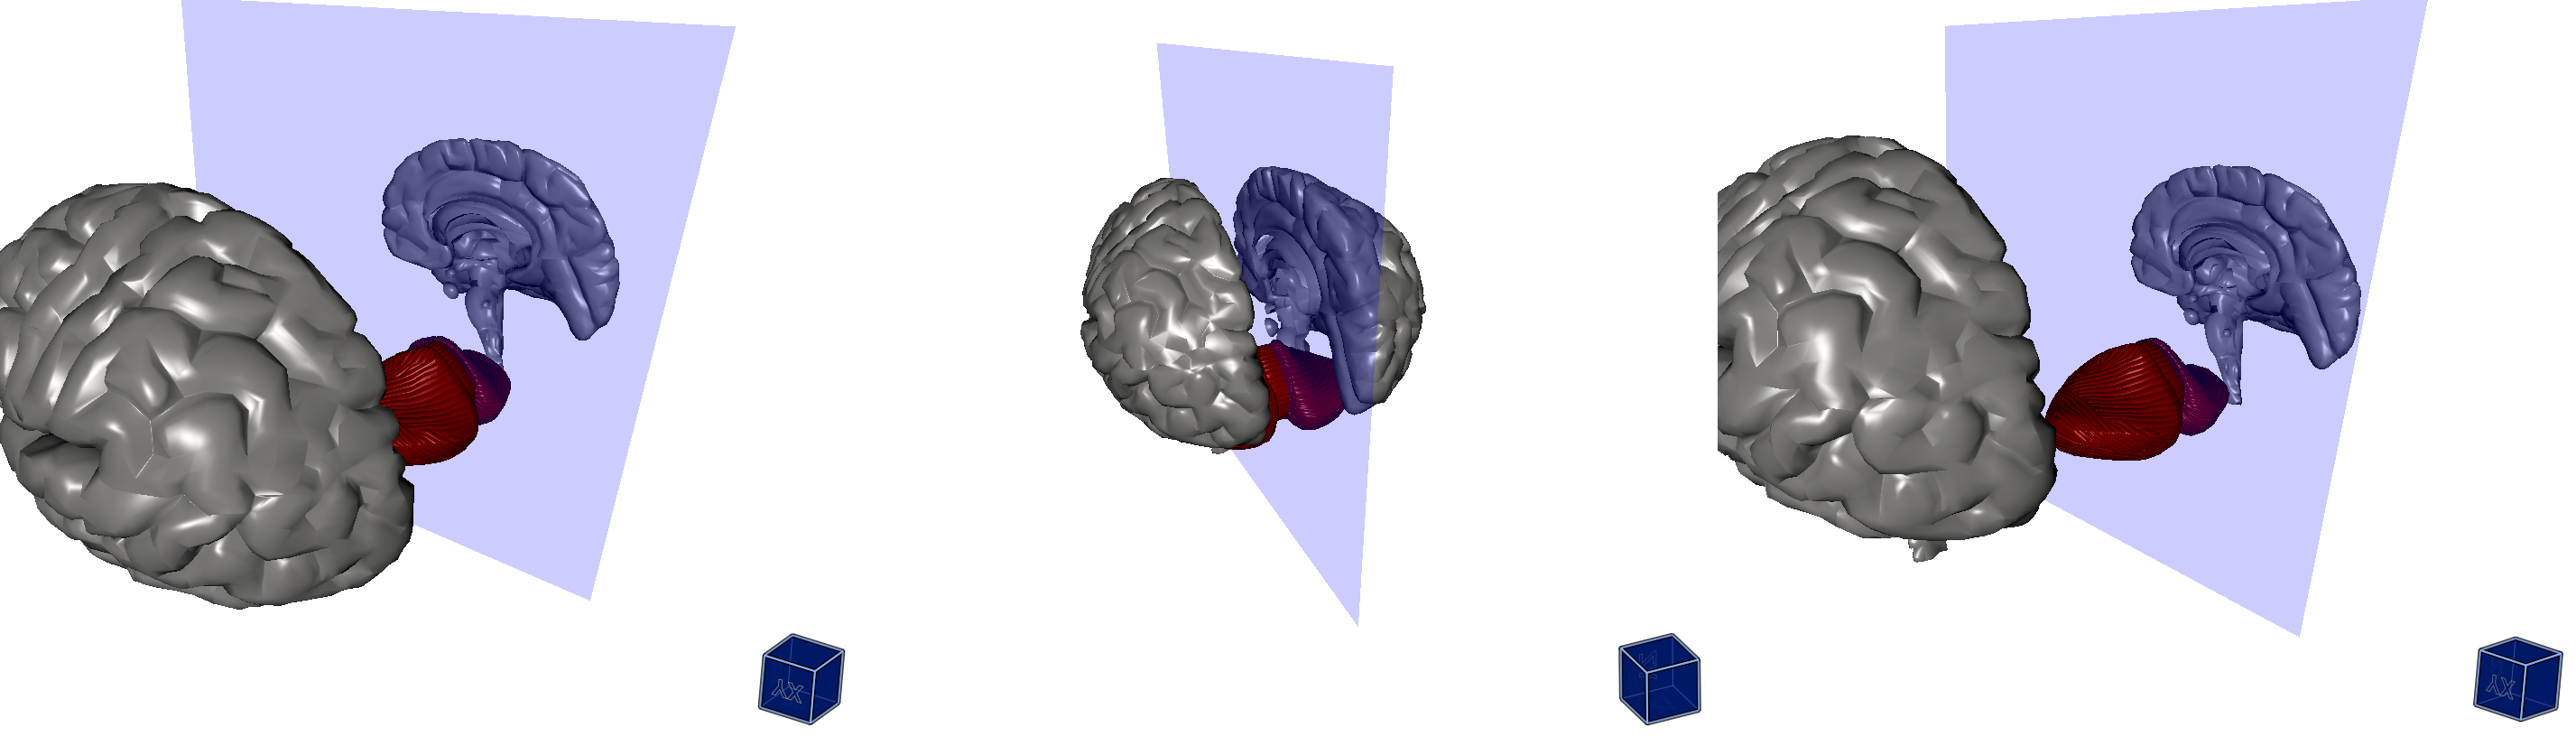
\includegraphics[width=0.9\textwidth]{chapters/figures/cerebellum}
	\caption{Exploded view of a brain with the offset of the displaced halves are set amanually}
	\label{fig:cerebellum}
\end{figure}

\subsection{Milestone 2: find a safe distance, find a split plane} 
The next step would be to automatically place the two halves of the object so that they would not collide with the object of interest and to find a suiting plane to split the object.\\
As I was aiming for an animated transition between offsets, I chose an implicit approach to finding the ideal offset of the two halves:\\
Each time the object would be rendered I would first render the three parts (Object of interest, front half, back half) with the low-cost overlay shader counting the rendered pixels of the non-occluded object ($p_{unoccluded}$), counting the amount of pixels drawn using openGL occlusion queries and during the actual rendering counting the amount of pixels drawn with possible occlusions ($p_{occluded}$). The ratio $r$ determined by
\begin{equation}\label{eq:Occlusion ratio}
	r =\frac{p_{unoccluded} - p_{occluded}}{ p_{unoccluded}}
\end{equation}
for
\begin{equation}
	p_{occluded} \neq 0
\end{equation}

is multiplied with the speed specified by user input resulting in the speed at which the offset grows toward an ideal offset which is the maximum offset described in Milestone 3 or an offset of 0 if the difference between  ($p_{unoccluded}$) and  ($p_{occluded}$) is 0 with the ideal offset different than the maximum offset.\\
Because the ratio tends towards 0 the more the object is revealed the growth of the offset diminishes the more is revealed , coming to a halt as soon as the whole object is fully revealed which is the moment the ideal offset is set to the current offset.\\
%\begin{verbatim}
%float ratio_selected = occlusions[0]- occlusions[1];
%	if (ratio_selected>0){
%	ratio_selected/=occlusions[0];
%	if (ghosting){
%		ideal_offset[0]=boundsDiameter;
%		ideal_offset[1]=-boundsDiameter;
%	}else{
%		ideal_offset[0]=20.0f;
%		ideal_offset[1]=-20.0f;
%	}
%	speed=GetPlugin().GetProperty("Speed");
%	speed*=ratio_selected;
%}else{
%	//stop
%	}
%\end{verbatim}
This movement is akin to the movement of the object being pulled by a spring toward the point of full revelation of the object of interest, though not a linear spring, because the change of speed is determined by the amount of Pixels that are revealed in each iteration making the spring constant proportional to $r$.
To avoid that the Object still moves at very low speeds, resulting in huge amounts of unnecesary costly redraws,I introduced a  minimum speed $\epsilon$ so that the object comes to a halt earlier.\\

\subsection{Milestone 3: Optimize Distance, force-field animation of split, optimize fringe distance cases} 

The objective of this last Milestone is to give a smooth appearance to the graphic while the view is changed by User interaction. The first step is to make the transition between two offsets smooth with the transition speed $s$ proportional to $\Delta_{offset}$
\begin{equation}
	s=s_u \cdot \Delta_{offset}
\end{equation}
thus creating a movement with linear deceleration that comes to a halt when the ideal offset is reached. this behaviour can be observed if the option ``Dynamic Offset `` is deactivated.\\
With dynamic ratio turned on and the object of interest is (partially) occluded the ideal offset is set to the maximum  offset and speed $s$ is multiplied by the ratio $r$ described in milestone 2 so that when the split parts move away from the object of interest the movement halts when the whole object is fully revealed setting the current offset as the ideal offset.\\
In case the object is revealed and the explosion needs to be collapsed the ideal offset is set to 0.0 until the object of interest is no longer fully visible, in which case the movement ideal offset is set to maximum and now grows outwards as described before.\\
This creates a visualization that smoothly adapts to new viewing points and changes in the splitting plane, but has one major disadvantage:\\
If a plane normal on either side of the plane points approximately in the same direction as the viewing vector,  the offset needed to reveal the whole object of interest become very huge in comparison to the object itself. This may prove fatal to the expressiveness of the visualization, given that the goal is to represent an object in context of the parts that are exploded, but the distance between the components is either so large that parts of the components partially move outside of the screen or even completely outside or behind the viewing plane or it is necessary to zoom out or move the camera back so that the whole object is visible causing substantial loss of detail, due to the large offset. If the $\vec{planeNormal} \cdot \vec{viewingVector} = \pm1$ or the object has a certain shape (e.g large at the end in direction of the offset, see  \ref{fig:infinity}
) the offset would even grow to infinity.\\
\begin{figure}[tb]
	\centering
	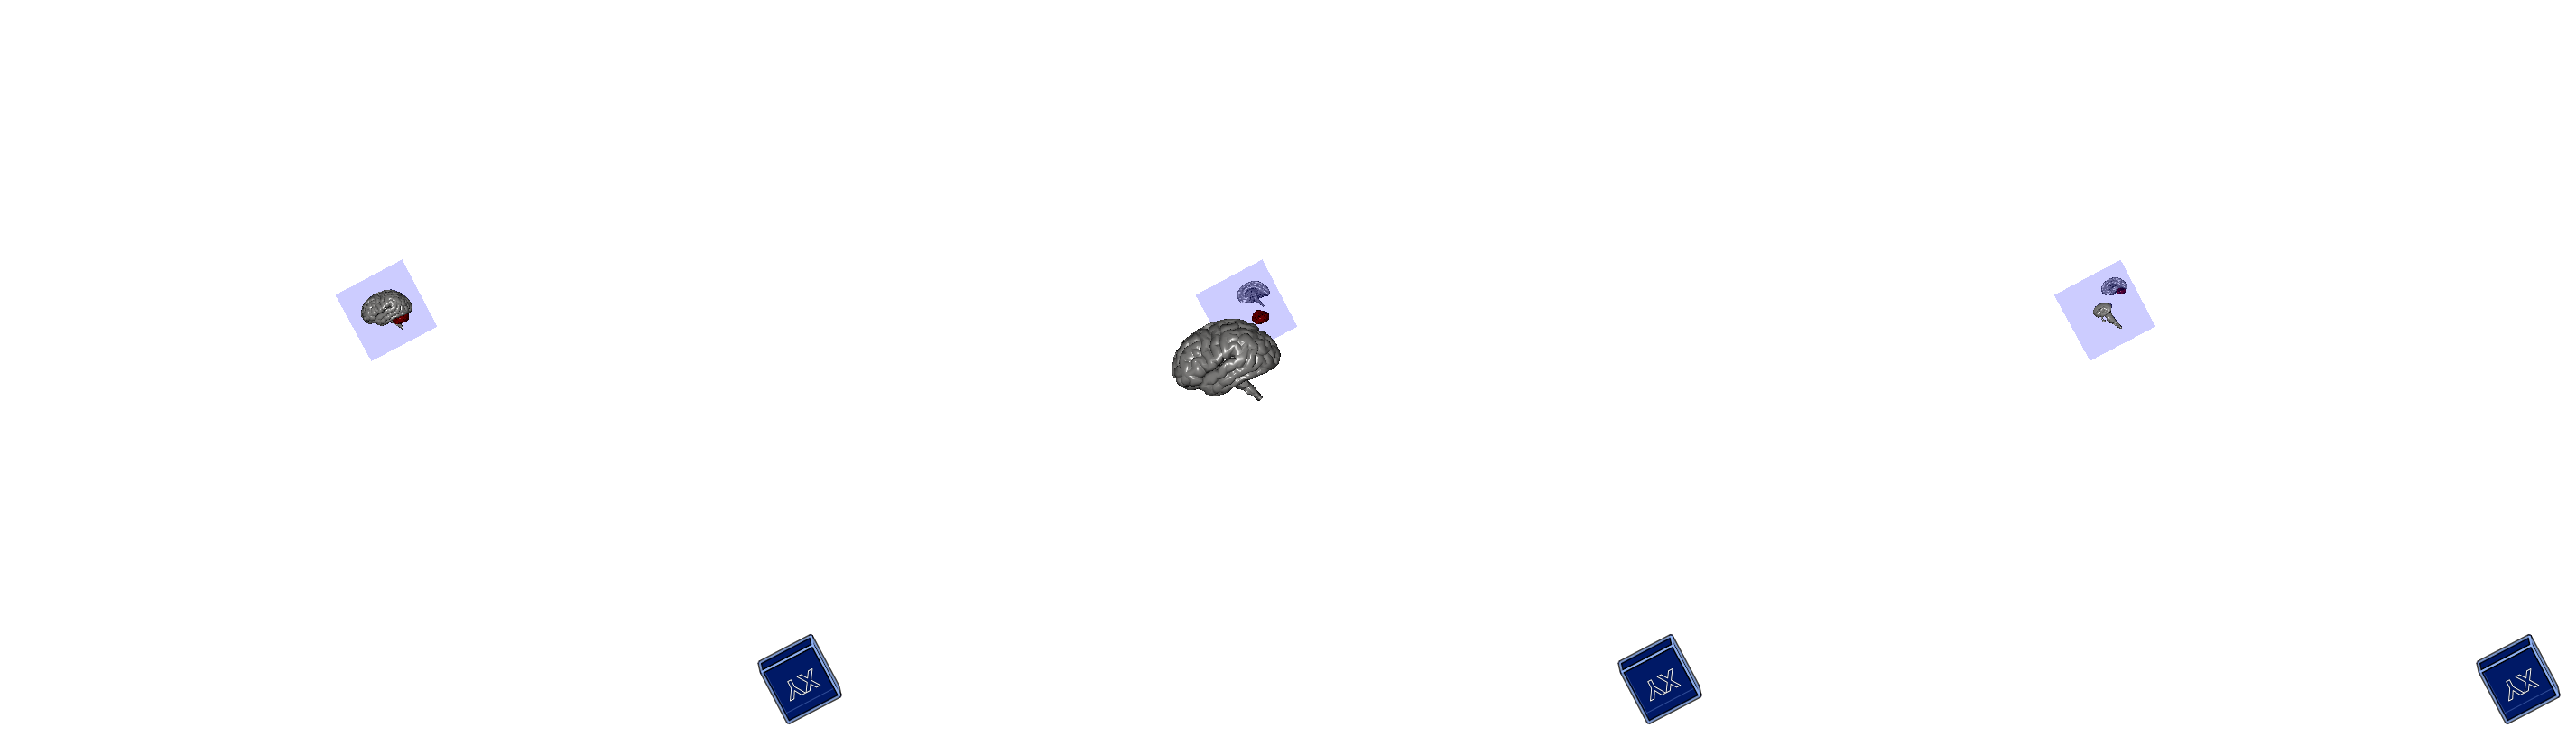
\includegraphics[width=0.9\textwidth]{chapters/figures/infinity}
	\caption{Different objects of interest from roghly the same viewpoint caus the offset to grow, placing the object out of view}
	\label{fig:infinity}
\end{figure}
To circumvent this problem I defined a maximum offset $o_{max}$ of the objects diameter which is the length of the distance between the minimum and maximum corners of the bounding box of the mesh. Since the mesh itself has no bounding box, the bounding box has to be accumulated by combining the bounding boxes of the groups of the mesh. This way the distance between the exploded parts can never exceed twice the diameter of the object.\\
To avoid parts of the object of interest now being occluded I used a simple ghosting technique: 
The front part, meaning the exploded part that is between the viewer and the split plane, is being rendered translucently if the distance becomes too large.
If the current offset $o_c$ exceeds $o_{max} \cdot 0.7$ the opacity $\alpha$ of the front part is linearly interpolated between $1.0$ at $o_c = o_{max} \cdot 0.7$ and $0.5$ at  $o_c = o_{max}$ using the formula
\begin{equation}
	\alpha = \frac{o_{max}-o_c}{o_{max} \cdot 0.3} \cdot 0.5 + 0.5
\end{equation}
This opacity factor $\alpha$ is then multiplied by $r$ so that the object stays solid while its not occluding anything and is most translucent if the whole object of interest is occluded completely.\\
To determine which part is the front part, I calculated the dot product of the viewing vector and the plane normal, using its sign to determine whether the part shifted in direction of the plane normal is the front part or not. This also determines in which order the parts are rendered, with the front part being the last, so that it can be translucently blended over the solid parts.\\
A problem that now appears is that backface culling is deactivated to so that the cutaway can be rendered correctly, resulting in the translucent objects' backfaces also visible, which causes the graphic to appear slightly confusing and aesthetically unpleasant. This can be avoided by allowing backface culling for a translucent object, if its offset vector doesn't point away from the camera. Because this may be the case if the camera is placed between the original and the translated switch plane, the dot product has to be calculated once more, now for the translated split plane.\\
\begin{figure}[tb]
	\centering
	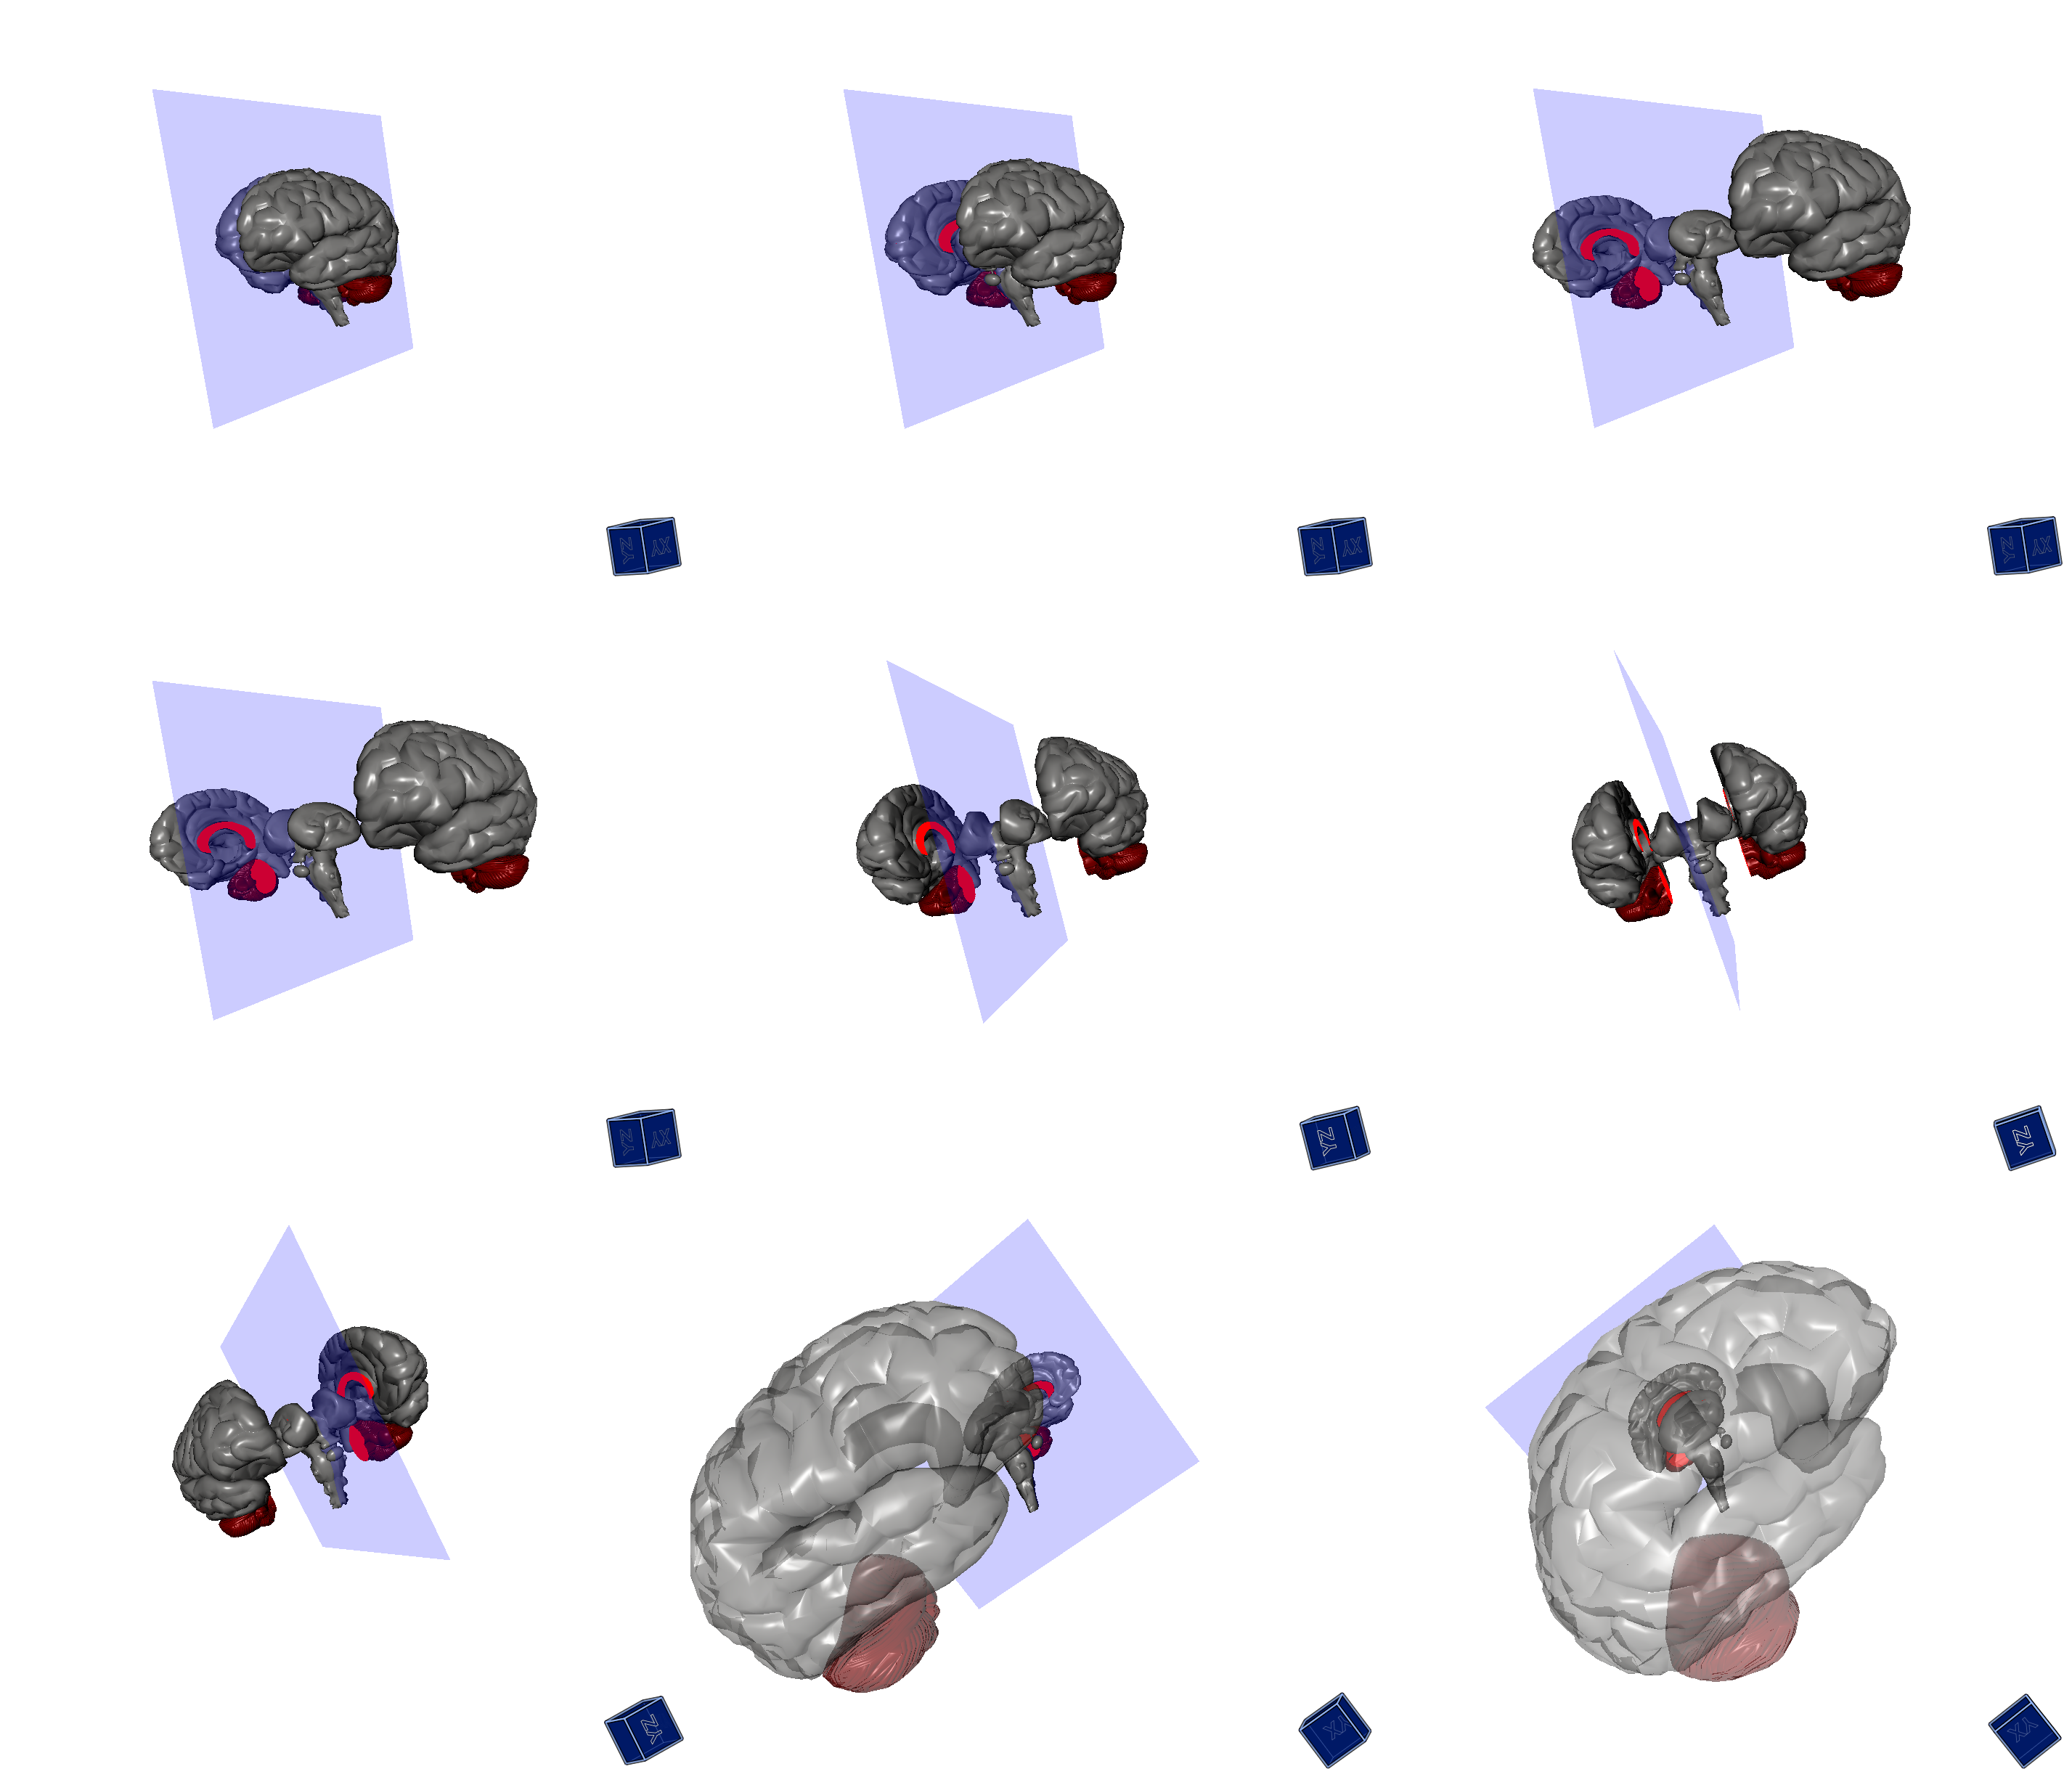
\includegraphics[width=0.9\textwidth]{chapters/figures/brainstem}
	\caption{Depiction of the animations and ghosting in the final version of the plugin}
	\label{fig:brainstem}
\end{figure}
\chapter{Conclusion}
In general I think that the combination of ghosting and exploded views in this form is not an ideal one, 